\documentclass{article}
\usepackage{amsmath,amssymb,graphicx,geometry,tikz,
            array,booktabs,enumitem,listings,xcolor,hyperref}
\geometry{margin=1in}
\hypersetup{colorlinks=true,linkcolor=blue,urlcolor=blue}

\title{Module 7: Multiclass Linear Prediction, Generalization, and Distribution Shift}
\author{Machine Learning Course}
\date{}

\begin{document}
\maketitle
\tableofcontents
\newpage

%%%%%%%%%%%%%%%%%%%%%%%%%%%%%%%%%%%%%%%%%%%%%%%%%%%%%%%%%%%%%%%%%%%%
\section{Introduction}
Multiclass supervised learning demands both accurate prediction
and formal guarantees that the accuracy will persist on future data.
This module ties \emph{three} linear models
(multiclass Perceptron, soft-margin SVM, multinomial logistic regression)
to the statistical-learning framework, shows how \emph{margin size}
controls sample complexity, and discusses what happens
when the train/test distributions drift apart.

%%%%%%%%%%%%%%%%%%%%%%%%%%%%%%%%%%%%%%%%%%%%%%%%%%%%%%%%%%%%%%%%%%%%
\section{Mathematical Framework}\label{sec:SLT}
Let the instance space be $\mathcal{X}\subseteq\mathbb{R}^{d}$,
label space $\mathcal{Y}=\{1,\dots,k\}$,
and $P$ the unknown joint distribution on $\mathcal{X}\!\times\!\mathcal{Y}$.
Given a training sample
$S=\{(x^{(i)},y^{(i)})\}_{i=1}^{n}\stackrel{\text{i.i.d.}}{\sim}P$,
the goal is to select a hypothesis $h:\mathcal{X}\!\to\!\mathcal{Y}$
minimising the \textit{true error}
\[
\operatorname{TrueErr}(h)=
\Pr_{(x,y)\sim P}\!\bigl[h(x)\neq y\bigr].
\]
We can only observe the \textit{training error}
$\operatorname{TrainErr}_{n}(h)$.
Finite-sample guarantees take the form
\[
\Bigl|\operatorname{TrainErr}_{n}(h)-\operatorname{TrueErr}(h)\Bigr|
\;\le\;
\sqrt{\frac{c(\mathcal{H})}{n}}
\]
with probability at least $1-\delta$,
where $c(\mathcal{H})$ is a complexity parameter
(VC dimension, log\,$|\mathcal{H}|$, Rademacher, etc.)
\cite{vapnik1998}.\\%
\fbox{\parbox{\dimexpr\textwidth-2\fboxsep-2\fboxrule}{%
\textbf{Homework link.}
Exercise 2 asks which photo-collection strategy respects
this i.i.d.\ assumption.
Training on images sampled \emph{across California}
best matches the test distribution,
hence minimises hidden covariate shift.}}

\subsection{Margin-based Bound}
For linear separators that classify all points with margin
$\gamma>0$ and radius $R$
$\bigl(\|x^{(i)}\|\le R\bigr)$,
one obtains
\[
c(\mathcal{H})\;\le\;\frac{R^{2}}{\gamma^{2}}
\quad(\text{independent of }d),
\]
explaining why large-margin SVMs can succeed in
extreme dimension-to-sample-ratio settings
\cite{bartlett1998}.\\%
\fbox{\parbox{\dimexpr\textwidth-2\fboxsep-2\fboxrule}{%
\textbf{Homework 7, Problem 3.}
Even with one million features and only 1000 points,
a large margin keeps $R^{2}/\gamma^{2}$ modest,
so the generalisation gap shrinks.}}

%%%%%%%%%%%%%%%%%%%%%%%%%%%%%%%%%%%%%%%%%%%%%%%%%%%%%%%%%%%%%%%%%%%%
\section{Multiclass Linear Predictors}\label{sec:models}
For each class $j$ store parameters $(w_{j},b_{j})\in\mathbb{R}^{d+1}$.
Define the score function
\[
f_{j}(x)=w_{j}^{\top}x+b_{j},
\qquad
\hat y=\arg\max_{j}f_{j}(x).
\]
Decision regions are convex polytopes separated by
$(w_{j}-w_{\ell})^{\top}x+(b_{j}-b_{\ell})=0$
\cite{crammer2001}.%

\subsection{Worked Boundary Example (Homework 1)}
Given
$w_{1}=(1,1),\,b_{1}=0$,
$w_{2}=(1,0),\,b_{2}=1$,
$w_{3}=(0,1),\,b_{3}=-1$,
the pairwise hyperplanes are
$y=1$, $x=-1$, and $y=x+2$.
Figure~\ref{fig:regions} diagrams the regions.
\begin{figure}[h]
\centering
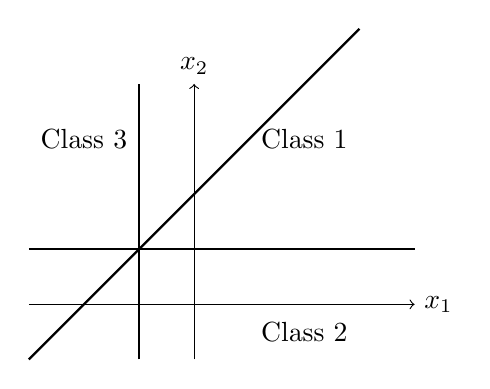
\begin{tikzpicture}[scale=0.7]
\draw[->] (-3,0)--(4,0) node[right] {$x_{1}$};
\draw[->] (0,-1)--(0,4) node[above] {$x_{2}$};
\draw[thick] (-3,1)--(4,1);
\draw[thick] (-1,-1)--(-1,4);
\draw[thick] (-3,-1)--(3,5);
\node at (2,3){Class 1};
\node at (2,-0.5){Class 2};
\node at (-2,3){Class 3};
\end{tikzpicture}
\caption{Decision regions for the boundary example.}
\label{fig:regions}
\end{figure}

%------------------------------------------------------------------
\subsection{Multiclass Perceptron}
\paragraph{Loss Function}
\[
\ell_{\text{perc}}((x,y);W)=
\begin{cases}
0 & f_{y}(x)\ge f_{j}(x)\;\forall j,\\
1 & \text{otherwise.}
\end{cases}
\]
\paragraph{Algorithm}
\fbox{\parbox{\dimexpr\textwidth-2\fboxsep-2\fboxrule}{%
\textbf{Multiclass Perceptron} (one pass)\newline
\textbf{input\;} data $(x^{(i)},y^{(i)})_{i=1}^{n}$, classes $1{:}k$\newline
Initialise $w_{j}\leftarrow 0,\;b_{j}\leftarrow 0$\newline
\textbf{for} $i=1$ to $n$:\newline
\phantom{00}predict $\hat y\leftarrow\arg\max_{j}(w_{j}^{\top}x^{(i)}+b_{j})$\newline
\phantom{00}\textbf{if} $\hat y\neq y^{(i)}$:\newline
\phantom{0000}$w_{y^{(i)}}\leftarrow w_{y^{(i)}}+x^{(i)}$, \;
$w_{\hat y}\leftarrow w_{\hat y}-x^{(i)}$\newline
\phantom{0000}$b_{y^{(i)}}\leftarrow b_{y^{(i)}}+1$, \;
$b_{\hat y}\leftarrow b_{\hat y}-1$}}
\paragraph{Convergence Theorem}
If there exist parameters with margin $\gamma>0$ on data
$\|x^{(i)}\|\le R$, the total number of mistakes is
no more than $(R/\gamma)^{2}$ \cite{crammer2003}.

\subsection{Soft-Margin SVM (Crammer--Singer)}
\paragraph{Primal Problem}
\begin{align}
\min_{w_{j},b_{j},\xi}
&\;
\sum_{j=1}^{k}\|w_{j}\|_{2}^{2} + C\sum_{i=1}^{n}\xi_{i}
\\
\text{s.t. }&
f_{y^{(i)}}(x^{(i)})-f_{y}(x^{(i)})\ge 1-\xi_{i},
\quad
\forall i,\; \forall y\neq y^{(i)},\;
\xi_{i}\ge 0.
\nonumber
\end{align}
Variables $=kd+k+n$;
constraints $=n(k-1)$.
\paragraph{Margin/Complexity Trade-off}
Large $C$ penalises slack heavily,
yielding wider margins but potentially higher variance;
small $C$ allows violations, trading bias for variance.

\subsection{Multinomial Logistic Regression}
\paragraph{Softmax Model}
\[
p(y=j\mid x)=
\frac{\exp(f_{j}(x))}{\sum_{\ell=1}^{k}\exp(f_{\ell}(x))},
\qquad
\hat y=\arg\max_{j}f_{j}(x).
\]
\paragraph{Objective}
Minimise
$-\sum_{i=1}^{n}\log p(y^{(i)}\mid x^{(i)})$,
a convex function in $(w_{j},b_{j})$.
\paragraph{Calibration}
Reliability diagrams check whether predicted probabilities
match empirical frequencies; temperature scaling can correct mis-calibration.

%%%%%%%%%%%%%%%%%%%%%%%%%%%%%%%%%%%%%%%%%%%%%%%%%%%%%%%%%%%%%%%%%%%%
\section{Implementation Details}\label{sec:impl}
\subsection*{Quick Python Snippets}
\paragraph{Perceptron core}
\begin{lstlisting}[language=Python,basicstyle=\ttfamily\small]
def mc_perceptron(X, y, k, epochs=30):
    d = X.shape[1]
    W = np.zeros((k, d))
    b = np.zeros(k)
    for _ in range(epochs):
        for xi, yi in zip(X, y):
            scores = W.dot(xi) + b
            y_hat = scores.argmax()
            if y_hat != yi:
                W[yi] += xi
                W[y_hat] -= xi
                b[yi] += 1
                b[y_hat] -= 1
    return W, b
\end{lstlisting}

\paragraph{Crammer--Singer SVM via scikit-learn}
\begin{lstlisting}[language=Python,basicstyle=\ttfamily\small]
from sklearn.svm import LinearSVC
clf = LinearSVC(loss="hinge", multi_class="crammer_singer", C=1.0)
clf.fit(X_train, y_train)
\end{lstlisting}

%%%%%%%%%%%%%%%%%%%%%%%%%%%%%%%%%%%%%%%%%%%%%%%%%%%%%%%%%%%%%%%%%%%%
\section{Distribution Shift}\label{sec:shift}
\paragraph{Covariate Shift}
$P_{tr}(x)\neq P_{te}(x)$, but $P(y\mid x)$ fixed.
\emph{Importance weighting}: weight test loss by
$w(x)=\tfrac{P_{te}(x)}{P_{tr}(x)}$.

\paragraph{Label Shift}
$P_{tr}(y)\neq P_{te}(y)$, and $P(x\mid y)$ unchanged.
Estimate new class priors by moment-matching
$\hat\pi = (\mathbf{X}^{\top}\mathbf{X})^{-1}\mathbf{X}^{\top}\hat{q}$
where $\mathbf{X}_{ij}=p(x^{(i)}\mid y=j)$.\\

\fbox{\parbox{\dimexpr\textwidth-2\fboxsep-2\fboxrule}{%
\textbf{Homework 7, Problem 4 answers.}
(a) Different topic priors $\Rightarrow$ label shift.\;
(b) Same topics but vocabulary drift $\Rightarrow$ covariate shift.}}

%%%%%%%%%%%%%%%%%%%%%%%%%%%%%%%%%%%%%%%%%%%%%%%%%%%%%%%%%%%%%%%%%%%%
\section{Mathematical Justification}\label{sec:justify}
\subsection{Why Margin Helps Generalisation}
The margin bound
$R^{2}/\gamma^{2}$ arises from
bounding the growth function of half-spaces separated by margin
\cite{bartlett1998}.
Maximising the minimum margin (as SVM does)
directly shrinks the complexity term,
lowering required sample size.

\subsection{Why Perceptron Converges (Sketch)}
Let $u=\bigl[w_{1}^{*};\dots;w_{k}^{*}\bigr]$
be a reference separator with unit norm and margin $\gamma$.
Define global parameter vector $\theta$
by stacking all $w_{j}$.
Each mistake raises $u^{\top}\theta$ by at least $\gamma$
and increases $\|\theta\|$ by at most $R$.
After $M$ mistakes,
$\gamma M \le u^{\top}\theta \le \|\theta\| \le R\sqrt{M}$,
hence $M \le (R/\gamma)^{2}$.

%%%%%%%%%%%%%%%%%%%%%%%%%%%%%%%%%%%%%%%%%%%%%%%%%%%%%%%%%%%%%%%%%%%%
\section{Programming-Exercise Checklist}\label{sec:prog}
\begin{enumerate}[label=\arabic*.]
\item Draw decision regions on a $400\times400$ grid using
      \texttt{plt.contourf}.
\item Shuffle data after each Perceptron epoch; early-stop if no errors.
\item Train SVM for $C=0.01,0.1,1,10$ and
      plot four separate boundaries.
      Comment on margin width versus boundary jaggedness.
\end{enumerate}

%%%%%%%%%%%%%%%%%%%%%%%%%%%%%%%%%%%%%%%%%%%%%%%%%%%%%%%%%%%%%%%%%%%%
\section{Conclusion}
Perceptron, SVM, and logistic regression
share a common geometric core;
their differences lie in loss functions and regularisers.
Margin maximisation links simplicity to generalisation,
and understanding covariate versus label shift
is critical for reliable deployment.

%%%%%%%%%%%%%%%%%%%%%%%%%%%%%%%%%%%%%%%%%%%%%%%%%%%%%%%%%%%%%%%%%%%%
\bibliographystyle{plain}
\begin{thebibliography}{9}
\bibitem{vapnik1998}
Vladimir Vapnik.
\newblock \emph{Statistical Learning Theory}.
\newblock Wiley, 1998.%

\bibitem{bartlett1998}
Peter Bartlett and Philip Bartlett.
\newblock The Sample Complexity of Pattern Classification with Margin.
\newblock In \emph{IEEE Transactions on Information Theory}, 1998.%

\bibitem{crammer2001}
Koby Crammer and Yoram Singer.
\newblock On the Algorithmic Implementation of Multiclass Kernel-Based Vector Machines.
\newblock \emph{Journal of Machine Learning Research}, 2001.%

\bibitem{crammer2003}
Koby Crammer and Yoram Singer.
\newblock Ultraconservative Online Algorithms for Multiclass Problems.
\newblock \emph{Journal of Machine Learning Research}, 2003.%
\end{thebibliography}

\end{document}
